\documentclass[11pt,a4paper]{article}
\bibliographystyle{apalike}
\usepackage{epsfig, hyperref}
\usepackage{amsmath}
\usepackage{natbib}
\usepackage{listings}
\usepackage{color}

\definecolor{dkgreen}{rgb}{0,0.6,0}
\definecolor{gray}{rgb}{0.5,0.5,0.5}
\definecolor{mauve}{rgb}{0.58,0,0.82}

\lstset{frame=tb,
  language=Python,
  aboveskip=3mm,
  belowskip=3mm,
  showstringspaces=false,
  columns=flexible,
  basicstyle={\small\ttfamily},
  numbers=none,
  numberstyle=\tiny\color{gray},
  keywordstyle=\color{blue},
  commentstyle=\color{dkgreen},
  stringstyle=\color{mauve},
  breaklines=true,
  breakatwhitespace=true,
  tabsize=3
}

\begin{document}

\title{Python ``Cheat Sheet''}
\author{Nicholas P. Ross}
\date{\today}
\maketitle


% Usually omit these for ApJ or MNRAS style files:
%\tableofcontents
%\listoffigures
%\listoftables

\begin{abstract}
The is my (NPR's) version of a $\sim$Python ``Cheat Sheet'', 
(including some parts for folks that want to migrate form 
IDL). 
\end{abstract}

\section{Real basics}
    \subsection{iPython}
     \$ conda update ipython

    \subsection{Versions}
    \$ python3
    \begin{lstlisting}
    Python 3.5.2 (v3.5.2:4def2a2901a5, Jun 26 2016, 10:47:25) 
    [GCC 4.2.1 (Apple Inc. build 5666) (dot 3)] on darwin
    Type "help", "copyright", "credits" or "license" for more information.
    >>> import numpy 
    >>> print (numpy.__version__)
    1.11.1 

    >>> import astropy 
    >>> print (astropy.__version__)
    1.2.1 
 
    >>> import sys
    >>> print (sys.version)
    3.5.2 (v3.5.2:4def2a2901a5, Jun 26 2016, 10:47:25) 
    [GCC 4.2.1 (Apple Inc. build 5666) (dot 3)]

    \end{lstlisting}
 

    \subsection{iPython from Fernando Perez}
    Try: tmpnb.org  {\bf VERY USEFUL}\\
    \href{http://www.pythonforbeginners.com/basics/ipython-a-short-introduction}{http://www.pythonforbeginners.com/basics/ipython-a-short-introduction}

    \subsection{Notebook}
    Click on the NBviewer...\\
    Then you can see the e.g. html of the notebook. \\
    But to change/execute it, then all you have to do is click the download button...\\
    Then put it on gitHub/Dropbox etc...\\
    (I need to learn about ``Tmox'' and ``SCreen'' Terminal emulators...)\\
  
    \noindent
    {\bf Run a code cell using Shift-Enter} or \\
    Alt-Enter runs the current cell and inserts a new one below.
    Ctrl-Enter run the current cell and enters command mode. 

    \noindent
    Google: ``ipython beyond plain python''\\
    
    http://nbviewer.ipython.org/github/fperez/cit2013/blob/master/06-IPython\%20-\%20beyond\%20plain\%20Python.ipynb

    iPython NB power = power of python + power of the command line with ``!'' + ``\%'' and ``\%\%'' ``magics''... 
    
http://nbviewer.ipython.org/github/ipython/ipython/blob/1.x/examples/notebooks/Part\%204\%20-\%20Markdown\%20Cells.ipynb

\begin{figure}
  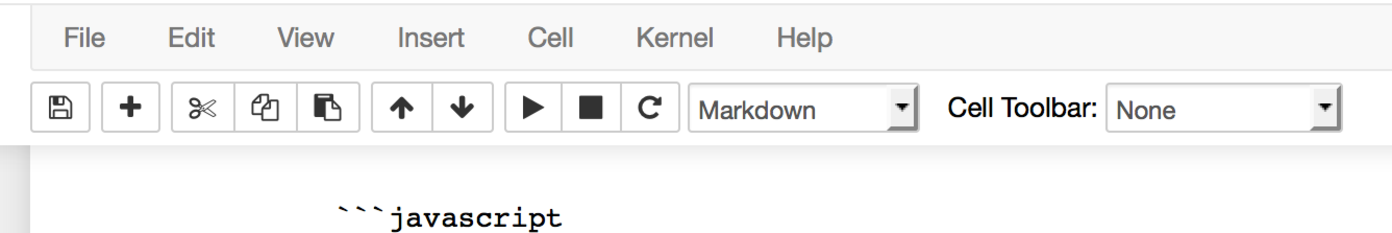
\includegraphics[height=4.0cm,width=14.0cm]
{iPython_NB_toolbar.pdf}
      \centering
      \caption[]
              {Clicking on the Cell Toolbar ``Code'', ``Markdown'' etc. will power what happens in the Clells!!!}
      \label{fig:fig1}
    \end{figure}

\href{https://github.com/profjsb/python-bootcamp}{https://github.com/profjsb/python-bootcamp}


\newpage
\section{Data Types}

\begin{lstlisting}
>>> n = 123
>>> f = 123.
>>> L = [1,2,3]
>>> a = (1,2,3)
>>> D = {1,2,3}
>>> s = '1,2,3'

>>> type(n)
<class 'int'>
>>> type(f)
<class 'float'>
>>> type(L)
<class 'list'>
>>> type(a)
<class 'tuple'>
>>> type(D)
<class 'set'>
>>> type(s)
<class 'str'>
\end{lstlisting}




\newpage
\section{Britton's Classes :-)}

\subsection{``If lost in the desert...''}
$>>>$ dir(thing) \\
$>>>$ dir(thing) \\

%% http://tex.stackexchange.com/questions/45981/square-brackets-in-math-mode-without-the-bracket-symbols

%%   Symbols in Python    % + - = ! / ( ) [ ] < > | ' :


\subsection{Lists}
\begin{lstlisting}
>>> super_list = [0, [3,4,5], "Hello World!", range(5)] 
>>> print super_list 

[0, [3, 4, 5], 'Hello World!', [0, 1, 2, 3, 4]] 
>>> print super_list[1] 
[3, 4, 5] 
>>> print super_list[-1]
[0, 1, 2, 3, 4] 
>>> print super_list[1[0]] 
Traceback (most recent call last):
  File "<stdin>", line 1, in <module>
TypeError: 'int' object is not subscriptable
>>> print super_list[1][0] 
  3

>>> c = range(10) 
>>> print c 
[0, 1, 2, 3, 4, 5, 6, 7, 8, 9]
>>> c.append(range(3)) 
>>> print c 
[0, 1, 2, 3, 4, 5, 6, 7, 8, 9, [0, 1, 2]]
>>> c.extend(range(3)) 
>>> print c 
[0, 1, 2, 3, 4, 5, 6, 7, 8, 9, [0, 1, 2], 0, 1, 2]
>>> del c[4]
>>> print c
[0, 1, 2, 3, 5, 6, 7, 8, 9, [0, 1, 2], 0, 1, 2]

>>> z =  [42]*5
>>> [42, 42, 42, 42, 42]

>>> print super_list
[0, [3, 4, 5], 'Hello World!', [0, 1, 2, 3, 4]]
>>> print len(super_list)
4
>>> print len(super_list[-1])
5
\end{lstlisting}


\subsection{Dictionaries and Maps}
From: \href{http://learnpythonthehardway.org/book/ex39.html}{http://learnpythonthehardway.org/book/ex39.html}: 
You are now going to learn about the Dictionary data structure in
Python. A Dictionary (or "dict") is a way to store data just like a
list, but instead of using only numbers to get the data, you can use
almost anything. This lets you treat a dict like it's a database for
storing and organizing data.

From: \href{https://docs.python.org/3/tutorial/datastructures.html\#dictionaries}{https://docs.python.org/3/tutorial/datastructures.html\#dictionaries}: 
Another useful data type built into Python is the dictionary (see
Mapping Types — dict). Dictionaries are sometimes found in other
languages as “associative memories” or “associative arrays”. Unlike
sequences, which are indexed by a range of numbers, dictionaries are
indexed by keys, which can be any immutable type; strings and numbers
can always be keys. Tuples can be used as keys if they contain only
strings, numbers, or tuples; if a tuple contains any mutable object
either directly or indirectly, it cannot be used as a key. You can’t
use lists as keys, since lists can be modified in place using index
assignments, slice assignments, or methods like append() and extend().

It is best to think of a dictionary as an unordered set of key: value
pairs, with the requirement that the keys are unique (within one
dictionary). A pair of braces creates an empty dictionary: {}. Placing
a comma-separated list of key:value pairs within the braces adds
initial key:value pairs to the dictionary; this is also the way
dictionaries are written on output.

The main operations on a dictionary are storing a value with some key
and extracting the value given the key. It is also possible to delete
a key:value pair with del. If you store using a key that is already in
use, the old value associated with that key is forgotten. It is an
error to extract a value using a non-existent key.

\begin{lstlisting}
# http://www.tutorialspoint.com/python/python_dictionary.htm
dict = {'Name': 'Zara', 'Age': 7, 'Class': 'First'}
print("dict['Name']: ", dict['Name'])
print("dict['Age']: ", dict['Age'])
print("dict['Alice']: ", dict['Alice]')
\end{lstlisting}

\noindent
From: \href{http://openbookproject.net/thinkcs/python/english3e/dictionaries.html}{http://openbookproject.net/thinkcs/python/english3e/dictionaries.html}:

Hashing. The order of the pairs may not be what was expected. Python uses complex algorithms, designed for very fast access, to determine where the key:value pairs are stored in a dictionary. For our purposes we can think of this ordering as unpredictable.
You also might wonder why we use dictionaries at all when the same concept of mapping a key to a value could be implemented using a list of tuples:
\begin{lstlisting}
>>> {"apples": 430, "bananas": 312, "oranges": 525, "pears": 217}
{'pears': 217, 'apples': 430, 'oranges': 525, 'bananas': 312}
>>> [('apples', 430), ('bananas', 312), ('oranges', 525), ('pears', 217)]
[('apples', 430), ('bananas', 312), ('oranges', 525), ('pears', 217)]
\end{lstlisting}

The reason is dictionaries are very fast, implemented using a
technique called hashing, which allows us to access a value very
quickly. By contrast, the list of tuples implementation is slow. If we
wanted to find a value associated with a key, we would have to iterate
over every tuple, checking the 0th element. What if the key wasn’t
even in the list? We would have to get to the end of it to find out.



\section{Key packages}
{\tt matplotib\\
numpy\\
scipy \\
ipython \\ 
pandas \\
sympy \\ 
nose \\
pyds9\\
pyFITS\\
yt\\
}

\section{Class vs. an Instance}
Difference between a class and an instance is an Object Oriented (OO)
concept.

Python and Ruby both recommend {\tt UpperCamelCase} for class names,
{\tt CAPITALIZED\_WITH\_UNDERSCORES} for constants, and {\tt
lowercase\_separated\_by\_underscores} for other names.  
%% see also https://en.wikipedia.org/wiki/Naming_convention\_(programming)

And {\tt snake\_case} for variable names, function names, and method names. 

Generally speaking, instance variables are for data unique to each instance and class variables are for attributes and methods shared by all instances of the class:

Definitions: 
from \href{http://www.tutorialspoint.com/python/python\_classes\_objects.htm}{http://www.tutorialspoint.com/python/python\_classes\_objects.htm}
\begin{itemize}
\item{Class: A user-defined prototype for an object that defines a set of
    attributes that characterize any object of the class. The attributes
    are data members (class variables and instance variables) and methods,
    accessed via dot notation.}

  %A blueprint defining the charactaristics and behaviors of an object of that class type. Class names should be written in CamelCase, starting with a capital letter.

\item{Instance variable: A variable that is defined inside a method
    and belongs only to the current instance of a class.}

\item{Inheritance: The transfer of the characteristics of a class to
    other classes that are derived from it.}
\end{itemize}



%Section heading
\section{IDL to Python}
Key links:\\
\href{http://www.johnny-lin.com/cdat_tips/tips_array/idl2num.html}{IDL to Numeric/numarray Mapping}\\
\href{http://www.astro.umd.edu/~mbk/idl-numpy.html}{NumPy for IDL users}\\

\href{http://mathesaurus.sourceforge.net/idl-numpy.html}{http://mathesaurus.sourceforge.net/idl-numpy.html}\\

\href{http://mathesaurus.sourceforge.net/idl-python-xref.pdf}{http://mathesaurus.sourceforge.net/idl-python-xref.pdf}\\

\begin{table}
  \begin{center}
    \setlength{\tabcolsep}{4pt}
    \begin{tabular}{ll}
      \hline\hline
      IDL code   & Python code \\
      \hline 
      .run 'foo.pro'  & exec(open("./findSecondLargestNo.py").read())\\
      \hline
      data=READFITS('file',header) 	 & data=pyfits.open('file')\\
      tdata  = mrdfits('SpIESch1ch2.fits',0, hdr) 	 & tdata = data[0].data \\
      tbdata = mrdfits('SpIESch1ch2.fits',1, hdr) 	 & tdata = data[1].data \\
      help, tbdata, /str     & info(tbdata)\\
      print, size(tbdata)  & shape(tbdata)\\
      print, tbdata[0].flux\_aper\_1 & print tbdata.FLUX\_APER\_1[0]\\
      help, tbdata.flux\_aper\_1        & tbdata.FLUX\_APER\_1? \\
      fluxaper = tbdata.flux\_aper\_1[2] & fluxaper = ??? \\
      \hline 
     {\it (using fitsio)} & d = fitsio.read('SpIESch1ch2.fits',1) \\
      \hline
      \label{tab:IDL2Python}
    \end{tabular}
    \caption{IDL to Python}
    \label{table:idl_vs_python}
  \end{center}
\end{table}



%%%%%%%%%%%%%%%%%%%%%%%%%%%%%%%%%%%%%%%%%%%
%%%%%%%%%%%%%%%%%%%%%%%%%%%%%%%%%%%%%%%%%%%
%%
%%      I N P U T
%%
%%%%%%%%%%%%%%%%%%%%%%%%%%%%%%%%%%%%%%%%%%%
%%%%%%%%%%%%%%%%%%%%%%%%%%%%%%%%%%%%%%%%%%%
\newpage
\section{INPUT}
Just some general ways to get variables read-in and different 'tricks' to Python3 input. \\
\href{https://en.wikibooks.org/wiki/Non-Programmer\%27s\_Tutorial\_for\_Python\_3/File\_IO}{https://en.wikibooks.org/wiki/Non-Programmer\%27s\_Tutorial\_for\_Python\_3/File\_IO}\\
\href{http://www.programiz.com/python-programming/file-operation}{http://www.programiz.com/python-programming/file-operation}\\
\href{http://stackoverflow.com/questions/3925614/how-do-you-read-a-file-into-a-list-in-python}{http://stackoverflow.com/questions/3925614/how-do-you-read-a-file-into-a-list-in-python}\\


\begin{lstlisting}
>>> s = eval(input())
>>> s = input().split()
asdf asdfasdf ddddf aa
>>> s
['asdf', 'asdfasdf', 'ddddf', 'aa']
\end{lstlisting}

\begin{lstlisting}
>>> x, y, z, n = int(eval(input())), int(eval(input())), int(eval(input())), int(eval(input()))
>>> x, y, z, n = (int(eval(input())) for _ in range(4))
\end{lstlisting}

\begin{lstlisting}
# Would like some code to read in .dat files...
with open('million_nos.dat') as f:
    lines = f.read().splitlines()
\end{lstlisting}

\begin{lstlisting}
data = [line.strip() for line in open("million_nos.dat", 'r')]
## Still need to test this...
\end{lstlisting}

%% # Would like some code to read in .csv files...
%% # Would like some code to read in .txt files...




%%%%%%%%%%%%%%%%%%%%%%%%%%%%%%%%%%%%%%%%%%%
%%%%%%%%%%%%%%%%%%%%%%%%%%%%%%%%%%%%%%%%%%%
%%
%%      O U T P U T
%%
%%%%%%%%%%%%%%%%%%%%%%%%%%%%%%%%%%%%%%%%%%%
%%%%%%%%%%%%%%%%%%%%%%%%%%%%%%%%%%%%%%%%%%%
\newpage
\section{OUTPUT}
For the ``write'' statement, I think you have to put everything into 
a string format, otherwise it just barfs... \\
\href{http://learnpythonthehardway.org/book/ex16.html}{http://learnpythonthehardway.org/book/ex16.html}

\noindent
\begin{lstlisting}
import random

size = 1000000
lis = random.sample(range(size), size)

outfile = open('temp.dat', 'w')
for i in range(len(lis)):
    outfile.write(str(lis[i])+'\n')
    
outfile.close()
\end{lstlisting}

\begin{lstlisting}
  outfile = open('WISE_spectra_triples_4wget_temp.dat', 'w') \\
  for i in range(len(ra)): 
    print i, ra[i] 
    plate_out = str(plate[i])
    mjd_out = str(mjd[i]) 
    fiberid_out = str(fiberid[i])

    outfile.write(plate_out+"/spec-"+plate_out+"-"+mjd_out+"-"+fiberid_out.zfill(4)+".fits \n")
\end{lstlisting}







\section{IDL Where...}


\section{v2 vs. v3}
\href{https://docs.python.org/3.0/library/2to3.html}{https://docs.python.org/3.0/library/2to3.html}\\
\href{https://docs.python.org/3/howto/pyporting.html}{https://docs.python.org/3/howto/pyporting.html}\\
\href{https://docs.python.org/3/howto/pyporting.html}{https://docs.python.org/3/howto/pyporting.html}
\href{https://docs.python.org/2/library/2to3.html}{https://docs.python.org/2/library/2to3.html}\\
\$ {\tt 2to3 -w example.py}\\


    \subsection{print}
    {\tt print a} vs. {\tt print (a)}
    Thus, just use () all the time!!
    
    \subsection{Division}
    / = truncating (integer floor) division in P2.x when using ints; float division in P3.x
    // = truncating div in P2.x, P3.x 
    

\section{Linear Algebra}
\href{http://docs.scipy.org/doc/scipy/reference/tutorial/linalg.html}{http://docs.scipy.org/doc/scipy/reference/tutorial/linalg.html}

\begin{lstlisting}
import numpy as np
from scipy import linalg
A = np.array([[1,2],[3,4]])
linalg.inv(A)
A.dot(linalg.inv(A)) #double check
\end{lstlisting}

\noindent
\href{https://twitter.com/SciPyTip/status/756510468160774144}{https://twitter.com/SciPyTip/status/756510468160774144}
You can solve a linear system {\bf Ax = b} with {\tt linalg.solve(A, b)}.
\begin{lstlisting}

\end{lstlisting}



\section{Gotchas}
``follow up: PYTHONPATH is a hazardous environment variable, and should never include one Python's site-packages'' 
%% <blockquote class="twitter-tweet" lang="en"><p><a href="https://twitter.com/npr247">@npr247</a> <a href="https://twitter.com/jakevdp">@jakevdp</a> <a href="https://twitter.com/demitrimuna">@demitrimuna</a> follow up: PYTHONPATH is a hazardous environment variable, and should never include one Python\&#39;s site-packages</p>\&mdash; Min RK (@minrk) <a href="https://twitter.com/minrk/status/555137558850453505">January 13, 2015</a></blockquote><script async src="//platform.twitter.com/widgets.js" charset="utf-8"></script>

See 429 in history\_20150113.txt and onwards... :-) 

%> echo \$PYTHONPATH 
%:/Users/npr1/boss/products/Darwin/sdss3tools/v1_7_4/python:/cos_pc19a_npr/BOSS/esutil/esutil/lib/python2.7/site-packages/:/cos_pc19a_npr/BOSS/pydl/:/Users/npr1/boss/products/eups/bin



\newpage
\section{A few General Notes}
    \subsection{What's the difference between raw\_input() and input()?}
    The difference is that {\tt raw\_input()} does not exist in Python 3.x,
    while {\tt input()} does. Actually, the old {\tt raw\_input()} has been renamed to
     {\tt input()}, and the old  {\tt input()} is gone (but can easily be simulated by
    using  {\tt eval(input())}).
    Reference: \href{http://stackoverflow.com/questions/4915361/whats-the-difference-between-raw-input-and-input-in-python3-x}{http://stackoverflow.com/questions/4915361/whats-the-difference-between-raw-input-and-input-in-python3-x}. 
   

    \subsection{Loops}
    \begin{lstlisting}
   n = eval(input())
   for _ in range(n):
      <indented code here>
  \end{lstlisting}


    \subsection{List Comprehensions}
    \begin{lstlisting}
   >>> ListOfNumbers = [ x for x in range(10) ] # List of integers from 0 to 9
   >>> ListOfNumbers

   >>> ListOfThreeMultiples = [x for x in range(100) if x % 3 == 0] # Multiples of 3 below 10
   >>> ListOfThreeMultiples
   [0, 3, 6, 9, 12, 15, 18, 21, 24, 27, 30, 33, 36, 39, 42, 45, 48, 51, 54, 57, 60, 63, 66, 69, 72, 75, 78, 81, 84, 87, 90, 93, 96, 99]
   >>> 
  \end{lstlisting}  


    \subsection{String Manipulation}
    \begin{lstlisting}
  s = 'abababababababababab'
  >>> print(*s)
  a g a f g a s d g a s d f a s d f a s d f a s d f a s d f
  >>> type(s[1::2])
  <class 'str'>
  >>> s[::2]
  'aaaaaaaaaa'
  >>> s[1::2]
  'bbbbbbbbbb'
  >>> 
  \end{lstlisting}  

    \subsection{Array Manipulation}
    \begin{lstlisting}
   >>> arr = [1,2,3,4]
   >>> print(arr[::1])
   [1, 2, 3, 4]
   >>> print(arr[::-1])
   [4, 3, 2, 1]
   >>> print(" ".join(map(str, arr[::1])))
   1 2 3 4
   >>> print(" ".join(map(str, arr[::-1])))
   4 3 2 1
  \end{lstlisting}  



 
\section{A few general notes and commands}
    \subsection{join()}
    Description: The method {\tt join()} returns a string in which the string elements of sequence have been joined by str separator.\\
    Syntax: Following is the syntax for {\tt join()} method: {\tt str.join(sequence)}. \\
    Parameters: sequence -- This is a sequence of the elements to be joined. \\
    Example: 
    \begin{lstlisting}
   s = "-";
   seq = ("a", "b", "c"); # This is sequence of strings.
   print s.join( seq )
   a-b-c
  \end{lstlisting}

    \subsection{eval()}  
    The eval function lets a python program run python code within itself.
    \begin{lstlisting}
   x = 1
   eval('x + 1')
   2
   eval('x')
   1
  \end{lstlisting}
    \begin{lstlisting}
   l
   [5, 5]
   cmd
   'insert(0,5)'
   eval("l."+cmd)
   print l
  [5, 5, 5]
  \end{lstlisting}

    \subsection{map()}  
    {\tt map(function, iterable, ...)} \\
    Return an iterator that applies function to every item of iterable, yielding the results.
    \begin{lstlisting}
   >>> def cube(x): return x*x*x
   ... 
   >>> map(cube,range(1,11))
   <map object at 0x101c182e8>
   >>> list(map(cube,range(1,11)))
   [1, 8, 27, 64, 125, 216, 343, 512, 729, 1000]
   >>> 
  \end{lstlisting}
    The {\tt list()} is needed in Python 3.x. 

    \begin{lstlisting}
   def f(x): return x % 2 != 0 and x % 3 != 0
   ... 
   >>> filter(f,range(2,25))
   <filter object at 0x101c18390>
   >>> list(filter(f,range(2,25)))
   [5, 7, 11, 13, 17, 19, 23]
   >>> 
  \end{lstlisting}


    \subsection{strip()}  
    \begin{lstlisting}
   >>> str = "0000000this is string example....wow!!!0000000";
   >>> print (str.strip( '0' ))
   this is string example....wow!!!
  \end{lstlisting}

    \subsection{exec()}  
    Run whole programs from the python3 command prompt (see also~\ref{table:idl_vs_python}
    \begin{lstlisting}
   >>> exec(open("./findSecondLargestNo.py").read())
  \end{lstlisting}


\newpage
\section{Statistics}
 \begin{lstlisting}
 >>> import statistics as s
 >>> s.mean([1, 2, 3, 4, 4])
 2.8
 \end{lstlisting}


 

\section*{General Wee Tips}
Need points that are evenly spaced on a log scale? Use {\tt np.logscale(start, stop, base)} \\
By convention, matplotlib is imported as mpl. Also by convention, matplotlib.pyplot is imported as plt.\\




\section*{Useful Resources}
Borrows, begs and steals from: \\

\subsection*{General Python Resources}
http://docs.python.org/3.5/tutorial/\\
http://docs.scipy.org/doc/numpy/reference/routines.array-manipulation.html\\
http://www.scipy-lectures.org/intro/numpy/numpy.html\\
https://sites.google.com/site/aslugsguidetopython/\\
https://sites.google.com/site/aslugsguidetopython/data-analysis/array-manipulation\\

\subsection*{Inter-active links}
http://interactivepython.org/runestone/static/pythonds/SortSearch/TheBubbleSort.html\\
http://pythoncentral.io/time-a-python-function/\\


\subsection*{Teaching yourself Python}
http://www.tutorialspoint.com/python/\\
http://www.tutorialspoint.com/python/python\_classes\_objects.htm\\
http://codingbat.com/python\\
https://wiki.python.org/moin/ProblemSets\\
https://www.hackerrank.com/\\


\subsection*{IDL to Python}
http://www.astro.umd.edu/$sim$mbk/idl-numpy.html\\
http://www.johnny-lin.com/cdat\_tips/tips\_array/idl2num.html\\
http://www.astrobetter.com/idl-vs-python/ \\
http://www.astrobetter.com/wiki/tiki-index.php?page=Python+Switchers+Guide \\
http://mathesaurus.sourceforge.net/\\
http://mathesaurus.sourceforge.net/idl-numpy.html\\
http://www.scicoder.org/mapping-idl-to-python/\\
http://mathesaurus.sourceforge.net/idl-python-xref.pdf\\


\noindent
http://www.thelearningpoint.net/computer-science/learning-python-programming-and-data-structures/learning-python-programming-and-data-structures--tutorial-15--generators-and-list-comprehensions\\
https://jeffknupp.com/blog/2014/06/18/improve-your-python-python-classes-and-object-oriented-programming/\\
http://learnpythonthehardway.org/\\
http://learnpythonthehardway.org/book/ex40.html\\


\noindent
Also, 
http://www.cv.nrao.edu/~aleroy/pytut/topic2/intro\_fits\_files.py

\noindent





\end{document}

